\documentclass[10pt,twocolumn,letterpaper]{article}

\usepackage{cvpr}
\usepackage{times}
\usepackage{epsfig}
\usepackage{graphicx}
\usepackage{amsmath}
\usepackage{amssymb}

% Include other packages here, before hyperref.

% If you comment hyperref and then uncomment it, you should delete
% egpaper.aux before re-running latex.  (Or just hit 'q' on the first latex
% run, let it finish, and you should be clear).
\usepackage[breaklinks=true,bookmarks=false]{hyperref}

\cvprfinalcopy % *** Uncomment this line for the final submission

\def\cvprPaperID{****} % *** Enter the CVPR Paper ID here
\def\httilde{\mbox{\tt\raisebox{-.5ex}{\symbol{126}}}}

% Pages are numbered in submission mode, and unnumbered in camera-ready
%\ifcvprfinal\pagestyle{empty}\fi
\setcounter{page}{1}
\begin{document}

%%%%%%%%% TITLE
\title{Object Detection and Its Implementation on Android Devices}

\author{Zhongjie Li\\
Stanford University\\
450 Serra Mall, Stanford, CA 94305\\
{\tt\small jay2015@stanford.edu}
% For a paper whose authors are all at the same institution,
% omit the following lines up until the closing ``}''.
% Additional authors and addresses can be added with ``\and'',
% just like the second author.
% To save space, use either the email address or home page, not both
\and
Rao Zhang\\
Stanford University\\
450 Serra Mall, Stanford, CA 94305\\
{\tt\small zhangrao@stanford.edu}
}

\maketitle
%\thispagestyle{empty}

%%%%%%%%% ABSTRACT
\begin{abstract}
Object detection is a very important task for different applications including autonomous driving, face detection, video surveillance, etc. CNN based algorithm could be a great solution for object detection with high accuracy. Besides, most current deep learning applications are running on servers or desktop computers. Considering there are a lot of mobile computing devices available, we implemented the CNN based object detection algorithm on Android devices. The model architecture is based on SqueezeNet and further improved to find bounding boxes for recognized objects. The total model size is around 8 MB and makes it run fast, especially on mobile devices.

\end{abstract}

%%%%%%%%% BODY TEXT
\section{Introduction}
Deep learning based object detection has been very successful in recent years. Especially the CNN (convolutional neural network) model has significantly improved the recognition accuracy on large dataset. For the ImageNet benchmark data set, the CNN based model has been dominating the leaderboard since it's introduced by Krizhevsky in 2012 for the first time. 


While CNN based model can achieve higher accuracies, they have following disadvantages:

\begin{itemize}
    \item \textbf{High computation cost. } The CNN based model are usually very deep and each layer takes a lot of computation.
    \item \textbf{Large memory demand. } The CNN based model has a lot of parameters that usually take hundreds of Megabytes of memory space.
    \item \textbf{Low efficiency. } Most CNN based model are not designed for efficiency.
\end{itemize}

As mobile computing devices are very popular and comparatively powerful, people want to embrace the benefits of CNN with their mobile devices. However, to enable their mobile application,
new CNN architectures need to be developed to overcome the above issues.
Also, most deep learning frameworks have provided interface for mobile platforms, including iOS and Android. In this paper, we developed a CNN based model and then implemented it with Tensorflow and Android.


Our model is trained with KITTI benchmark. The KITTI data-set has over 100 GBytes of well-labeled data for object detection purpose. After training, our model is able to detect objects in view of camera on the Android device.

The rest of this paper is organized in the following order. Section 2 lists the related work of CNN architectures as well as CNN for object detection, discusses the state-of-the-art progress in CNN model compression. In Section 3, our model based on SqueezeDet is represented and elaborated. Section 4 introduces details of the KITTI data-set and the features to be used for our model. In Section 5, we conduct experiments with our proposed model and analyze the results from the experiments. Section 6 concludes our work and our future work is stated in Section 7.



%-------------------------------------------------------------------------
\section{Related Work}
In this section, we talk about CNN related work in object detection and the trend towards smaller CNN models.

\subsection{CNN Architectures}
Convolutional Neural Network (CNN) usually stands for the neural network which contains one or more convolutional neural layers. Each neural layer can be regarded as a combination of several spatial filters. These filters are used for extracting features from pictures. Some well-known filters are Histogram of Oriented Gradients (HOG) and color histograms, etc. A typical input for an convolutional layer is a 3-dimensional grid. They are height (H), width (W) and channels (C). Here each channel represents a filter in the convolutional layer. The input of first layer usually has a shape of (H, W, 3), where 3 stands for the RGB channels for the raw pictures.

CNN became popular in visual recognition field when it is introduced by LeCun \etal for handwritten zip code recognition~\cite{lecun1989backpropagation} in the late 90s. In their work, they used (5, 5, C)-size filters. Later work proved that smaller filters have multiple advantages, such as less parameters and reducing the size of network activations. In a VGG network~\cite{simonyan2014very} proposed by Karen Simonyan~\etal, (3, 3, C)-size filters are extensively used, while the networks such as Network-in-Networ~\cite{lin2013network} and GoogLeNet~\cite{szegedy2015going} widely adopt (1, 1, C)-size filters, the possibly smallest filters and used for compressing volume of the networks.

With the networks go deep, the filter size design gradually become a problem that almost all the CNN practitioners have to face. Hence, several schemes for network modularization are proposed. Such modules usually include multiple convolutional layers with different filter sizes and these layers are combined together by stack or concatenation. In a GoogLeNet architecture, such as~\cite{szegedy2015going, szegedy2016rethinking}, (1, 1, C)-size, (3, 3, C)-size and (5, 5, C)-size are usually combined together to form an "Inception" module and even with filter size of (1, 3, C) or (3, 1, C).

In addition to modularizing the network, communication and connections across multiple layers also improve the performance of the network. This seems to be a similar idea with Long Short Term Memory (LSTM) or Gated Recurrent Unit (GRU) architecture in Recurrent Neural Network (RNN). Residual Network (ResNet)~\cite{he2016deep} and Highway Network~\cite{srivastava2015highway} adopted such ideas to allow connections to skip multiple layers. These "bypass" connections can effectively send back the gradients through multiple layers without any blocking in a backward propagation pass when necessary.

\subsection{CNN for Object Detection}
With the advancement of accuracy in image classification, the research for object detection also developed in a fast speed. Before 2013, feature extraction techniques such as~\cite{dalal2005histograms}, which proposed an combined application of HoG and SVM can achieve a high accuracy on the PASCAL data-set~\cite{everingham2010pascal}. In 2013, a fundamental revolution occurred in this field, which was caused by the introduction of Region-based Convolutional Neural Networks (R-CNN), proposed by Girshick and Ross. R-CNN firstly proposes possible regions for residing objects, then makes use of CNN to classify objects in these regions. However, these two independent operations require high computation and make it time-consuming. An modification of R-CNN is made by Girshick and Ross, which is called fast R-CNN~\cite{girshick2015fast}. This architecture integrate the two independent tasks into one multi-task loss function, which accelerates the computation of proposals and classification. Later, a more integrated version of R-CNN, namely the faster R-CNN~\cite{ren1506towards} was proposed by Ren \etal, which achieves more than 10x faster than the original R-CNN. A recent proposal, R-FCN~\cite{li2016r} with a fully convolutional layer as the final parameterized layer further shortens the computation time used for region proposals. 

R-CNN can be regarded as a cornerstone for the development of CNN for object detection. A large amount of work is based on this architecture and achieves great accuracy. However, a recent work shows that CNN based object detection can be even faster. YOLO (You Only Look Once)~\cite{redmon2016you} is such an architecture integrating region proposition and object classification into one single stage, which significantly contributes to simplification of the pipeline of object detection, as well as reduction of the total computation time.

\subsection{Toward Smaller Models}
With CNN goes deeper, more parameters need to be stored, which makes the model larger and larger. Deeper CNN and larger modules usually achieve a higher accuracy, but people wonder whether a small model can reach a similar accuracy as a large model. In this sub-section, we talk about several popular model compression techniques aiming to reduce the size of CNN models.

As we know, singular value decomposition (SVD) is widely used to reduce matrix dimensionality. It is also introduced to pre-trained CNN models~\cite{denton2014exploiting} to reduce model size. Another approach reported is Network Pruning~\cite{han2015learning}, proposed by Han \etal, which prunes the parameters below a certain threshold to construct a sparse CNN. Recently, Han \etal have further improved their approach and proposed a new approach, Deep Compression, together with their hardware design to accelerate the computation of CNN models. A recent research called SqueezeNet~\cite{iandola2016squeezenet} even reveals that a complex CNN model as AlexNet~\cite{krizhevsky2012imagenet} accuracy can be compressed to smaller than 0.5 Mbytes.

Here are two examples of model compression. The famous ImageNet winner VGG-19 model stores more than 500 Mbytes parameters, which achieves a top-5 accuracy of about 87\% on ImageNet, while the equally famous ImageNet winner GoogLeNet-v1 only contains about 50 Mbytes parameters, achieving the same accuracy as VGG-19. The well-known AlexNet~\cite{krizhevsky2012imagenet} model with a size of more than 200 Mbytes parameters, achieves about 80\% top-5 accuracy on ImageNet image classification challenge, while the SqueezeNet~\cite{iandola2016squeezenet} model with a much smaller size, about 4.8 Mbytes parameters, can also achieve that accuracy. We can anticipate that there is much room left for compressing these CNN models, to better fit them to portable devices.

\begin{figure*}[ht]
\begin{center}
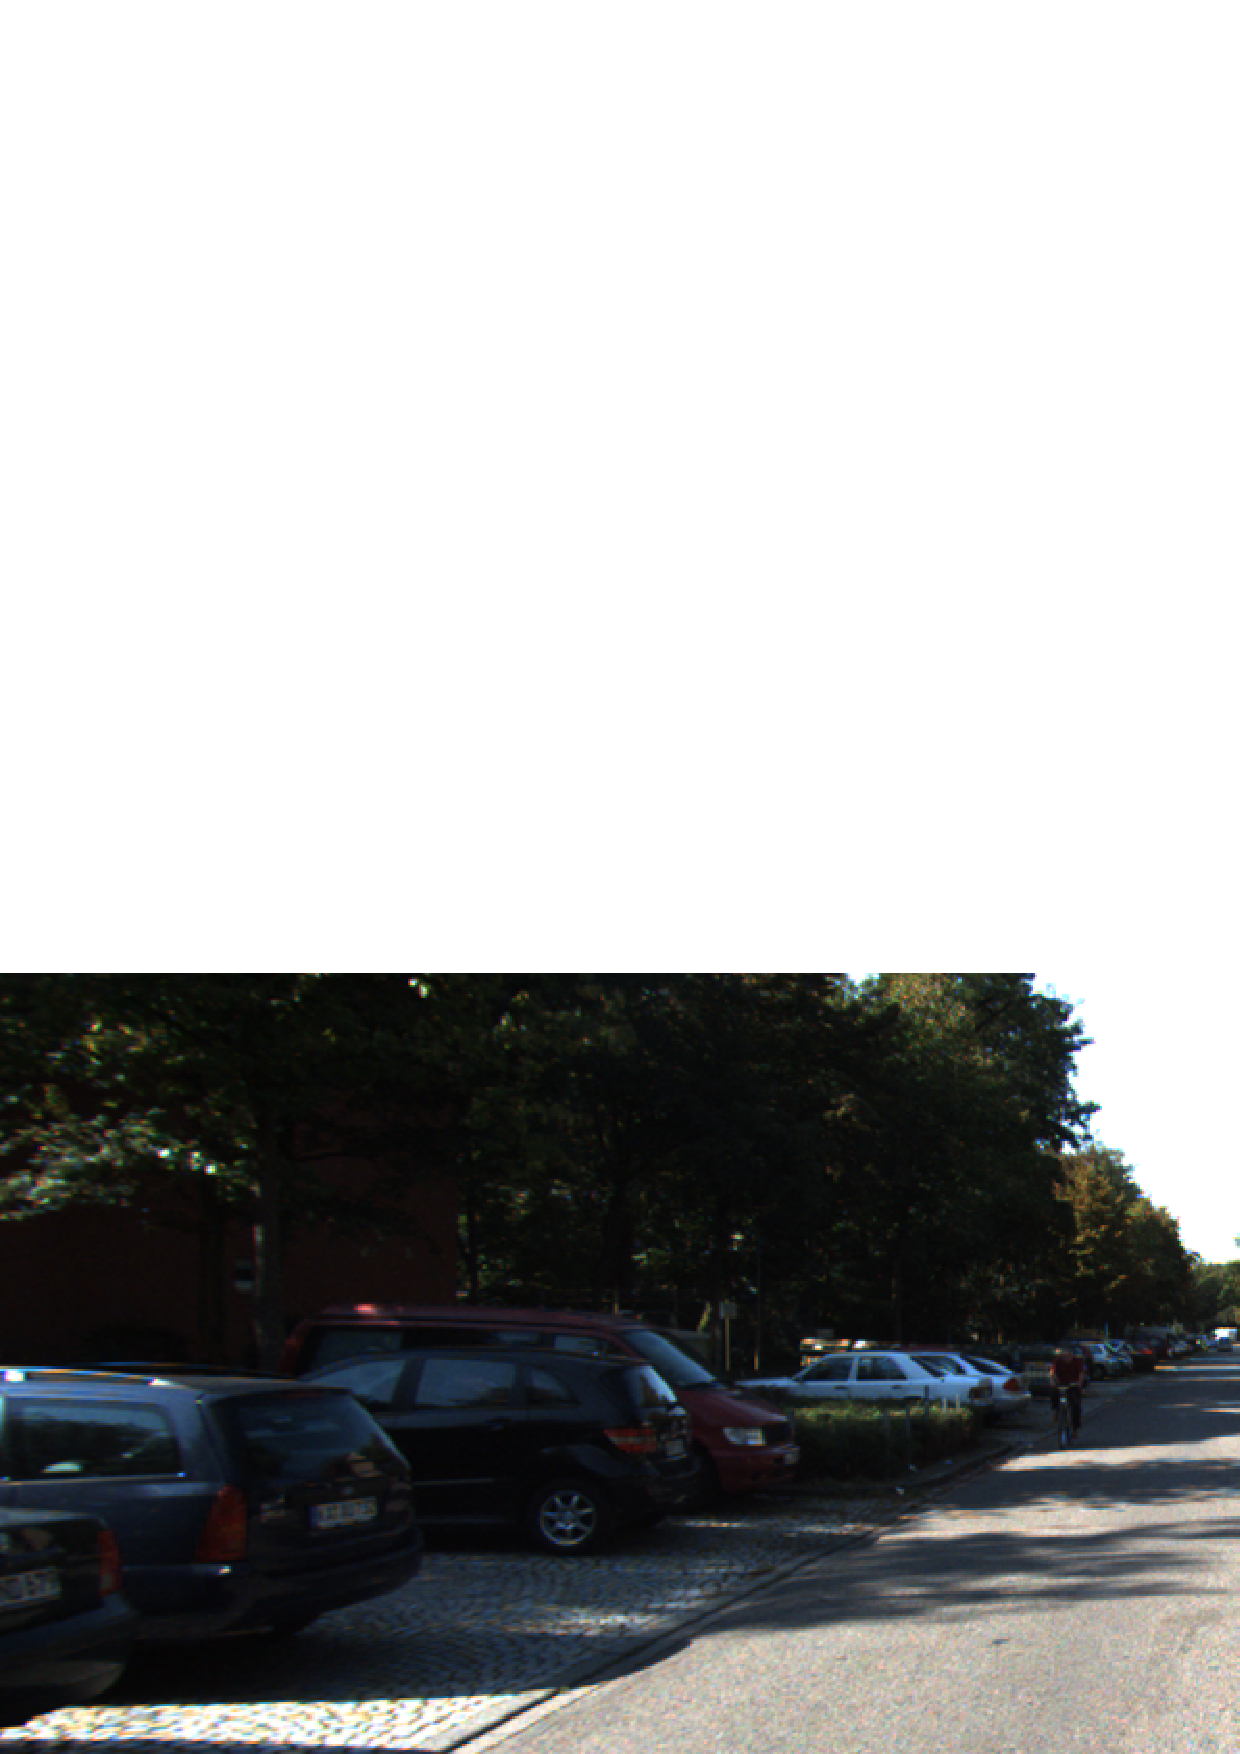
\includegraphics[width=1.0\linewidth]{fig/007480.png}
\end{center}
\caption{Example of A Picture in Data-set}
\label{fig:example}
\end{figure*}

\section{Methods}
As for the baseline, we implemented SqueezeDet model in an Android device. The SqueezeDet model is a fully convolutional neural network for object detection. It's based on SqueezeNet architecture that extract feature maps from image with CNN. Then another convolutional layer is used to find bounding boxes and class probabilities. The model has the benefit of small model size, good energy efficiency and goo accuracy due to the fact that it's fully convolutional and only contains a single forward pass.

For the implementation of CNN model in Android device, we used the interface provided by "Tensorflow Android Camera Demo". However, the interface is not well documented and it's designed for the specific application. The basic idea is to save the tensorflow graph and variables into a file after training the model. Then load the graph into Android device and evaluate operators' output with new input for the trained graph and variables in the Android application.



\section{Data-set and Features}
The data-set we use is The KITTI Vision Benchmark Suite\cite{geiger2012we}, which is made for academic use in the area of autonomous driving. For our target, we use the object detection data-set, which contains 7481 training images and 7518 test images. Total 80256 objects are labeled for this data-set and the 3 classes used for evaluation are cars, pedestrians and cyclists. The pictures in this data-set are fully color PNG files.\par
No pre-processing is done for the data-set, but data augmentation such as flipping and random cropping will be applied to increase the robustness of the network. Batch normalization will also be added to ameliorate the network initialization. Figure~\ref{fig:example} is an example picture in the KITTI data-set.

\section{Experiments}
The experiments include two parts. The first part is to examine the predicting accuracy of our CNN model against KITTI test data set. 
And the second part is to test the Android application in real world scenarios.
We expect to compare mean average precision (mAP), model size and detecting speed between different models. We will primarily focus on reducing model size and increasing detecting speed without losing much accuracy.

\section{Conclusion}
As a baseline, we have a running Android app that runs our CNN model trained by Tensorflow offline. The model size is ~8 MegaBytes and the testing accuracy is 76.7\%.
\section{Future Work}
Next step is to improve the Android application stability and functionality. In addition, we will improve the CNN model to further reduce the model size and improve the accuracy. 
\newpage

% \section{For reference}
% %------------------------------------------------------------------------
% \subsection{Table}
% \begin{table}
% \begin{center}
% \begin{tabular}{|l|c|}
% \hline
% Method & Frobnability \\
% \hline\hline
% Theirs & Frumpy \\
% Yours & Frobbly \\
% Ours & Makes one's heart Frob\\
% \hline
% \end{tabular}
% \end{center}
% \caption{Results.   Ours is better.}
% \end{table}



% %-------------------------------------------------------------------------
% \subsection{References}
% In such cases, include the
% anonymized parallel submission~\cite{Authors14}.

% Further details may be found
% in~\cite{Authors14b}, by Zeus \etal.

% The space after \eg, meaning ``for example'', should not be a
% sentence-ending space. So \eg is correct, {\em e.g.} is not.  The provided
% \verb'\eg' macro takes care of this.
% \cite{Alpher03,Alpher02,Authors14} to
% \cite{Alpher02,Alpher03,Authors14}.
% List and number all bibliographical references in 9-point Times,
% single-spaced, at the end of your paper. When referenced in the text,
% enclose the citation number in square brackets, for
% example~\cite{Authors14}.  Where appropriate, include the name(s) of
% editors of referenced books.


% %-------------------------------------------------------------------------
% \subsection{Illustrations, graphs, and photographs}

% \begin{figure*}
% \begin{center}
% 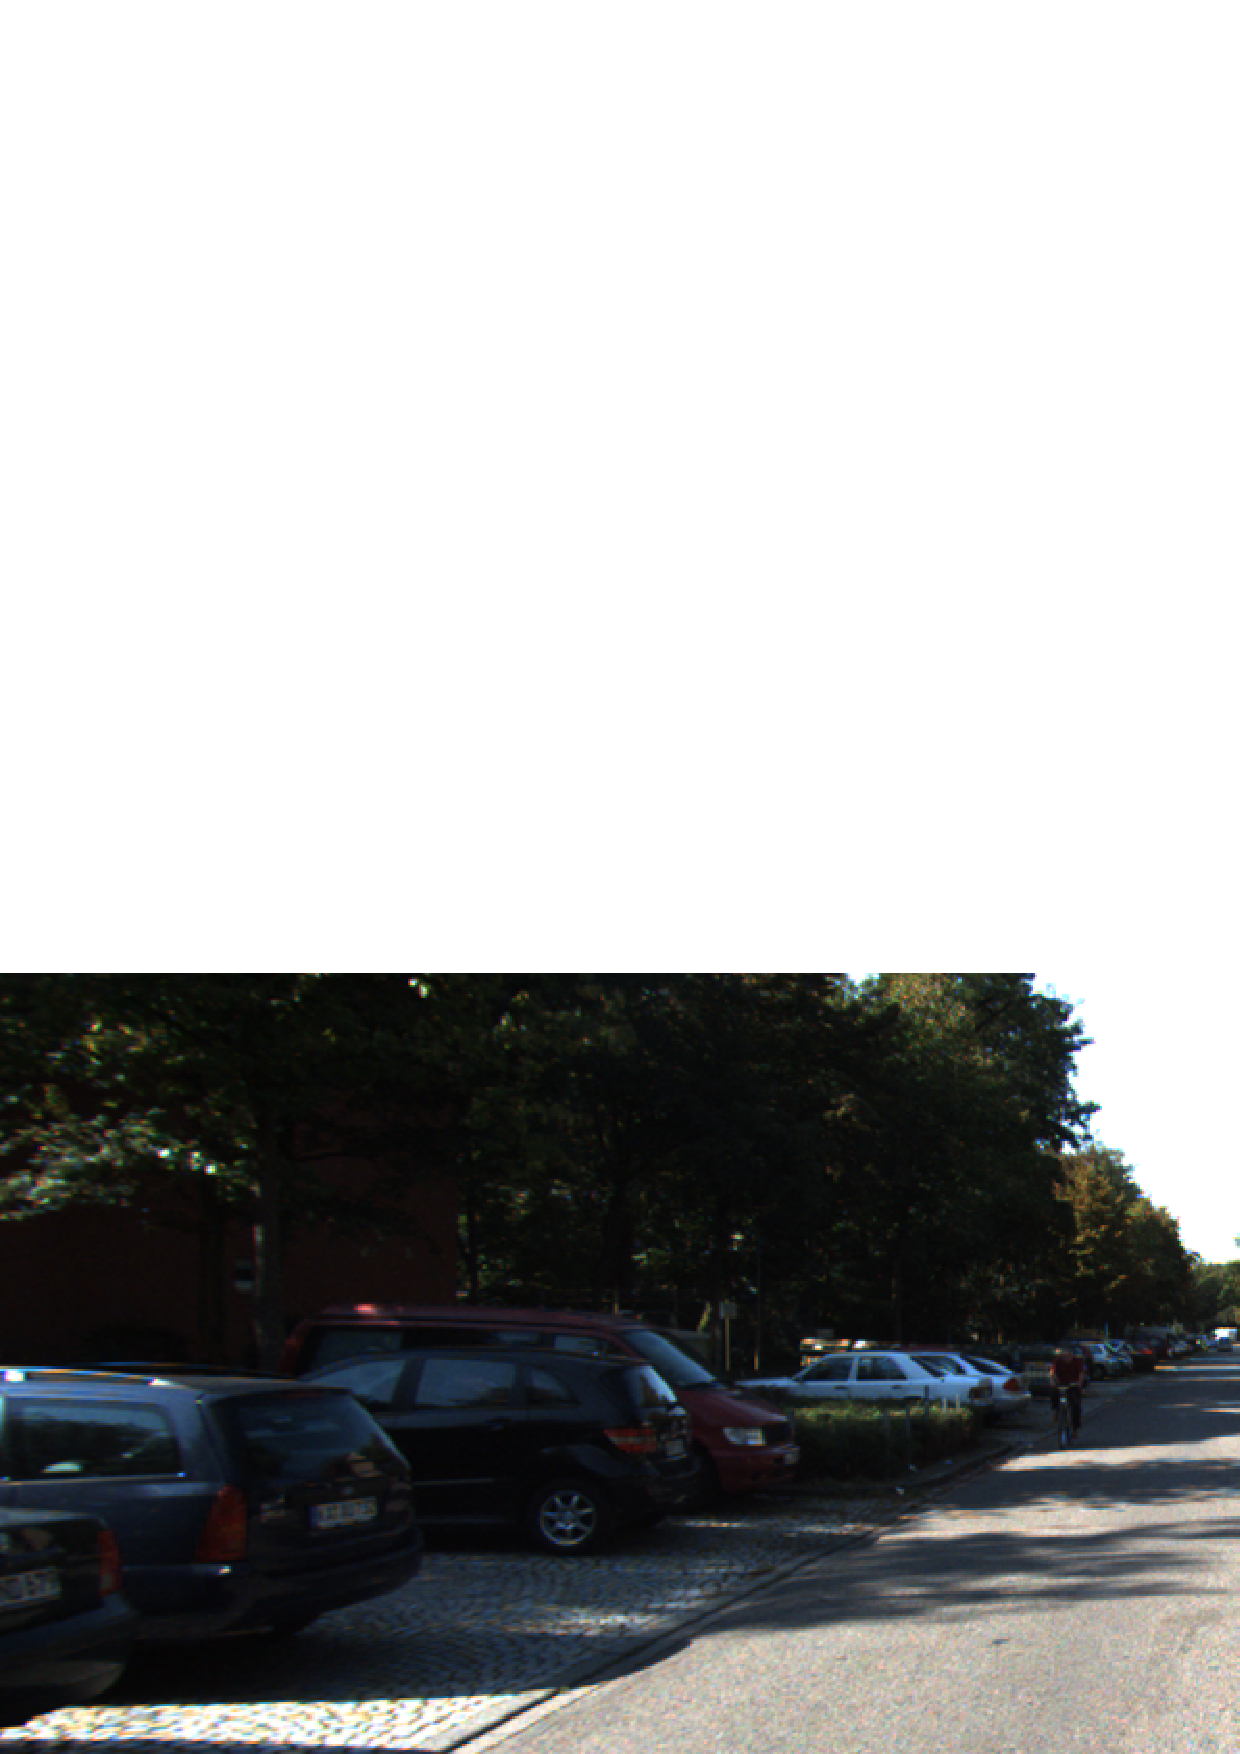
\includegraphics[width=0.8\linewidth]{fig/007480.png}
% \end{center}
% \caption{Example of Data-set}
% \label{fig:example}
% \end{figure*}

% Figures~\ref{fig:onecol} and~\ref{fig:short}.  Short captions should be centred.
% \begin{figure}[t]
% \begin{center}
% \fbox{\rule{0pt}{2in} \rule{0.9\linewidth}{0pt}}
%   %\includegraphics[width=0.8\linewidth]{egfigure.eps}
% \end{center}
%   \caption{Example of caption.  It is set in Roman so that mathematics
%   (always set in Roman: $B \sin A = A \sin B$) may be included without an
%   ugly clash.}
% \label{fig:long}
% \label{fig:onecol}
% \end{figure}


% When placing figures in \LaTeX, it's almost always best to use
% \verb+\includegraphics+, and to specify the  figure width as a multiple of
% the line width as in the example below
% {\small\begin{verbatim}
%   \usepackage[dvips]{graphicx} ...
%   \includegraphics[width=0.8\linewidth]
%                   {myfile.eps}
% \end{verbatim}
% }


{\small
\bibliographystyle{ieee}
\bibliography{egbib}
}




\end{document}
